\input ../../preamble.tex

\shortdate
\ddmmyyyydate

\begin{document}

\noindent
\fbox{\parbox{\textwidth}
{MAC6962: Tópicos Matemáticos para Computação Contemporânea
\hfill \formatdate{15}{10}{2019}
\vspace{3mm}
\begin{center}\LARGE 
Aula 4: Grafos aleatórios
\end{center}
\vspace{3mm}
{\em Professor: Yoshiharu Kohayakawa
\hfill
Aluno: Luiz Gabriel da Silva}
}}

\section{Aula 17 de Outubro de 2019}
\label{2019_10_17}

Esta nota de aula foi escrita por Vitor Santa Rosa Gomes, seguindo o conteúdo apresentado em aula por Yoshiharu Kohayakawa, com base principalmente no capítulo 5 de \cite[p.~245]{blum_hopcroft}, iniciado na aula anterior. As interpretações dadas são compiladas por Vitor podem não podem ser consideradas citações nem de Kohayakawa, nem de \cite{blum_hopcroft}.

% #region continuação teo5 caso ->infty
\subsection*{Relembrando o modelo GNP}

No modelo e grafos aleatórios $G\left(n,\ p\vphantom{1j}\right)$, $n$ é a quantidade de vértices no grafo e $p$ é a probabilidade de que uma aresta $vw$ esteja presente, independentemente das outras arestas. A seguir está a continuação do estudo da transição de fase do GNP quanto à sua conexidade.

\begin{teorema}
  No modelo $G\left(n,\ p\vphantom{1j}\right)$ de grafos aleatórios CNP, seja $n$ a quantidade de vértices e 
  \[
    p = \nicefrac{1}{n}\left(\log n + c_n\vphantom{1j}\right)
  \]
  a probabilidade de cada estar presente. Então
  \vspace*{-\baselineskip}
  \[
    \lim_{n\rightarrow\infty} \mathrm{P}\left[G\left(n,\ p\vphantom{1j}\right) \text{ é conexo}\vphantom{1j}\right] = \left\{\begin{array}{ll}
      0                               & \text{se } c_n\rightarrow-\infty                            \\
      \mathrel{e}^{-\mathrel{e}^{-c}} & \text{se } c_n\rightarrow c\in\mathds{R}                    \\
      1                               & \text{se } c_n\rightarrow\infty                             \\
    \end{array}\vphantom{1j}\right.
  \]
\end{teorema}

\subsection{Conexidade do CNP no caso $c_n\rightarrow\infty$}
\begin{proof}[Prova para o caso $c_n\rightarrow\infty$]
  Seja $X_k=\#$componentes de $G\left(n,\ p\vphantom{1j}\right]$ com $k$ vértices. Por exemplo, $X_1=\#$vértices isolados.

  Temos que a probabilidade do grafo ser desconexo em função da existência de vértices isolados é
  \vspace*{-\baselineskip}
  \begin{align*}
    \mathrm{P}\left[G\left(n,\ p\vphantom{1j}\right)\text{ é desconexo}\vphantom{1j}\right]
      &=    \mathrm{P}\left[\sum_{1\leq k\leq\nicefrac{n}{2}}X_k\geq 1\vphantom{1j}\right]
      \leq  \mathrm{E}\left[\sum_{1\leq k\leq\nicefrac{n}{2}}\vphantom{1j}X_k\right]                   \\
      &=    \sum_{1\leq k\leq\nicefrac{n}{2}}\mathrm{E}\left[X_k\vphantom{1j}\right]
      \leq  \sum_{1\leq k\leq\nicefrac{n}{2}}\binom{n}{k}\left(1-p\vphantom{1j}\right)^{k\left(n-k\vphantom{1j}\right)}.
  \end{align*}

  Quebrando a última expressão em duas parte, por manipulações algébricas, vale que
  \begin{align*}
    \sum_{1\leq k\leq n^{\nicefrac{3}{4}}}\binom{n}{k}\left(1-p\vphantom{1j}\right)^{k\left(n-k\vphantom{1j}\right)}
      &\leq \sum_{1\leq k\leq n^{\nicefrac{3}{4}}}\left(\nicefrac{\mathrm{e} n}{k}\cdot\mathrm{e}^{-p\left(n-k\vphantom{1j}\right)}\vphantom{1j}\right)^k  \\
      &\leq \sum_{1\leq k\leq n^{\nicefrac{3}{4}}}
              \left(\nicefrac{\mathrm{e} n}{k}\cdot\mathrm{e}^{-\log n-c_n+\smash{\overbrace{2\nicefrac{k}{n}\log n}^{o(1)}}}\vphantom{1j}\right)^k \\
      &\leq \sum_{1\leq k\leq n^{\nicefrac{3}{4}}}\left(\nicefrac{2}{k}\cdot\mathrm{e}^{1-c_n}\vphantom{1j}\right)^k
      \leq  3\mathrm{e}^{1-c_n} 
      \rightarrow 0
  \end{align*}

  e também vale que
  \begin{align*}
    \sum_{n^{\nicefrac{3}{4}}<k\leq\nicefrac{n}{2}}\binom{n}{k}\left(1-p\vphantom{1j}\right)^{k\left(n-k\vphantom{1j}\right)}
      &\leq \sum_{n^{\nicefrac{3}{4}}<k\leq\nicefrac{n}{2}}
              \left(\mathrm{e}\cdot\smash{\overbrace{\nicefrac{n}{k}}^{<n^{\nicefrac{1}{4}}}}\cdot
              \mathrm{e}^{\smash{\overbrace{-p\left(n-k\vphantom{1j}\right)}^{\geq\nicefrac{n}{2}}}}\vphantom{1j}\right)^k                             \\
      &\leq \sum_{n^{\nicefrac{3}{4}}<k\leq\nicefrac{n}{2}}\left(\mathrm{e}\cdot n^{\nicefrac{1}{4}}\cdot\mathrm{e}^{\nicefrac{-\log n}{2}}\vphantom{1j}\right)^k
      \leq  n^{\nicefrac{1}{5}\cdot n^{\nicefrac{3}{4}}}
      \rightarrow 0
  \end{align*}

  Em suma, 
  \[
    \mathrm{P}\left[G\left(n,\ p\vphantom{1j}\right)\text{ é desconexo}\vphantom{1j}\right] \rightarrow 0,
  \]
  o que é equivalente a dizer que
  \[
    \mathrm{P}\left[G\left(n,\ p\vphantom{1j}\right)\text{ é conexo}\vphantom{1j}\right] \rightarrow 1.
  \]
\end{proof}
% #endregion

% #region comentários sobre teo5 caso ->c
\subsection{Conexidade do CNP no caso $c_n\rightarrow c\in\mathds{R}$}

Este caso é similar aos anteriores, então seguem alguns comentários sobre a prova.

A partir do Teorema de Cayley sobre enumeração de árvores geradoras aleatórias de ordem $n$ --- <\href{https://en.wikipedia.org/wiki/Cayley%27s_formula}{https://en.wikipedia.org/wiki/Cayley\%27s\_formula}> ---, podemos usar a fórmula
\[
  \mathrm{E}\left[X_k\vphantom{1j}\right] = \binom{n}{k} \left(1-p\vphantom{1j}\right)^{k\left(n-k\vphantom{1j}\right)} k^{k-2} p^{k-1}.
\]

É útil algebricamente fazer a substituição:
\[
  k^{k-2} p^{k-1} = p\left(k\,p\vphantom{1j}\right)^{k-2} \rightarrow 0 \text{ se } k>2
\]

Como vimos no outro caso, em $c_n\rightarrow c$ quase não há componentes pequenas:
\[
  \mathrm{P}\left[G\left(n,\ p\vphantom{1j}\right)\text{ é desconexo}\vphantom{1j}\right] =
  \mathrm{P}\left[\sum_{k=2}^{\nicefrac{n}{2}} X_k \geq 1\vphantom{1j}\right] = \mathrm{E}\left[\sum_{k=2}^{\nicefrac{n}{2}} X_k\vphantom{1j}\right] \rightarrow 0.
\]

Concluímos que, com probabilidade que tende a $1$, $G\left(n,\ p\vphantom{1j}\right)$ é composto por uma componente e $X_1$ vértices isolados. Assim, falta agora estudar $X_1$: $G\left(n,\ p\vphantom{1j}\right)$ é conexo se e só se $X_1=0$.

\begin{fato}
  Vale que $X_1$ converge em probabilidade para uma variável aleatória $\mathrm{Poisson}\left(\mathrm{e}^{-c}\vphantom{1j}\right)$.
\end{fato}

Dado uma variável aleatória com distribuição \textit{Poison} $Z\sim\mathrm{Poisson}\left(\lambda\vphantom{1j}\right)$ (mais detalhes em <\href{https://en.wikipedia.org/wiki/Poisson_distribution}{https://en.wikipedia.org/wiki/Poisson\_distribution}>), valem as seguinets Propriedades:
\begin{itemize}
  \item $Z\in\mathds{N}$;
  \item $\mathrm{P}\left[Z=t\vphantom{1j}\right] = \mathrm{e}^{-\lambda}\cdot\nicefrac{\lambda^t}{t!}$, $t>0$;
  \item $\mathrm{E}\left[Z\vphantom{1j}\right] = \lambda$; e 
  \item $\mathrm{P}\left[Z=0\vphantom{1j}\right] = \mathrm{e}^{-c}$.
\end{itemize}

Pelo fato $X_1\sim\mathrm{Poisson}\left(\mathrm{e}^{-c}\vphantom{1j}\right)$ e pelas propriedades vistas, em particular para $X_1$ vale que
\[
  \mathrm{E}\left[X_1\vphantom{1j}\right]\rightarrow\mathrm{e}^{-c}
\]
assim como
\[
  \lim_{n\rightarrow\infty} \mathrm{P}\left[X_1=t\vphantom{1j}\right]
    = \mathrm{P}\left[\mathrm{Poisson}\left(\mathrm{e}^{-c}\vphantom{1j}\right)=t\vphantom{1j}\right]
    = \mathrm{e}^{-\mathrm{e}^{-c}}\,\nicefrac{\left(\mathrm{e}^{-c}\vphantom{1j}\right)^t}{t!}.
\]

Para todo $t$ fixo. Em particular,
\[
  \mathrm{P}\left[G\left(n,\ p\vphantom{1j}\right) \text{ é conexo}\vphantom{1j}\right] = \lim_{n\rightarrow\infty} \mathrm{P}\left[X_1=0\vphantom{1j}\right]=\mathrm{e}^{-\mathrm{e}^{-c}}
\]
%endregion

% #region teoB-Th87
\subsection{Teorema de Bollobás e Thomson}

O teorema abaixo é um resultado muito importante em grafos aleatórios, pois proporciona um esquema de prova para qualquer propriedade crescente, assim não é preciso buscar técnicas de prova específicas para conexidade, caminho Hamiltoniano, componentes grandes, entre outros.

\begin{definicao}
  Seja $\mathcal{P}$ uma propriedade de grafos e sejam $0\leq p\leq q\leq1$.

  Então a probabilidade de $G\left(n,\ q\vphantom{1j}\right)$ ter a propriedade $\mathcal{P}$ é pelo menos a probabilidade de $G\left(n,\ p\vphantom{1j}\right)$ ter a propriedade $\mathcal{P}$.
\end{definicao}

Descrevendo o teorema nos termos de função limiar da aula passada:

\begin{teorema}[B-Th'87]
  Seja $\mathcal{P}$ uma propriedade não trivial crescente. Então $\mathcal{P}$ admite uma função limiar:
  \vspace*{-\baselineskip}
  \begin{align*}
    \mathrm{P}\left[G_p\in\mathcal{P}\vphantom{1j}\right]
      &\rightarrow \left\{\begin{array}{ll}
                      0 & \text{se } p \ll p_0  \\
                      1 & \text{se } p \gg p_0  \\
                    \end{array}\vphantom{1j}\right. \\
    \mathrm{P}\left[G_p\not\in\mathcal{P}\vphantom{1j}\right]
      &\leq\epsilon
  \end{align*}
\end{teorema}

\begin{proof}
  Seja a função limiar $p_0<p_0\left(n\vphantom{1j}\right)$ tal que
  \[
    \mathrm{P}\left[G\left(n,\ p\vphantom{1j}\right)\in\mathcal{P} = \nicefrac{1}{2}\vphantom{1j}\right]
  \]

  Fixe $\epsilon>0$, e seja $t$ tal que $\left(\nicefrac{1}{2}\vphantom{1j}\right)t\leq\epsilon$. Considere $t$ cópias independentes de $G\left(n,\ p\vphantom{1j}\right)$, digamos $G_1,\ \ldots,\ G_t$. Seja $p'$ tal que $1-p'=(1-p_0)^t$.

  Considerando a seguinte partição do grafo,
  \[
    G\left(n,\ p'\vphantom{1j}\right) = G_1\cup\ldots\cup G_t
  \]

  temos que pela cota da união
  \[
    \mathrm{P}\left[G\left(n,\ p\vphantom{1j}\right)\not\in\mathcal{P}\vphantom{1j}\right]
      \leq \prod_{1\leq i\leq t} \mathrm{P}\left[G_i\not\in\mathcal{P}\vphantom{1j}\right]
      = \left(\nicefrac{1}{2}\vphantom{1j}\right)^t
      \leq \epsilon.
  \]

  Para o caso $p\gg p_0$, então
  \[
    \mathrm{P}\left[G\left(n, p\vphantom{1j}\right)\not\in\mathcal{P}\vphantom{1j}\right) \rightarrow 0
  \]
  pela definição da função limiar.

  Um argumento análogo prova que se $p\ll p_0$, então
  \[
    \mathrm{P}\left[G\left(n, p\vphantom{1j}\right)\in\mathcal{P}\vphantom{1j}\right) \rightarrow 0.
  \]
\end{proof}
% #endregion

% #region transição de fase em GNP
\subsection{Componente grande no GNP}

Existem outras formulações de grafos aleatórios além do $G\left(n,\ p\vphantom{1j}\right)$, porém foram descobertas formas de relacionar esses modelos entre si. Por exemplo, o modelo GT pode ser aproximado por um GNP $G_t\approx G\left(n,\ \nicefrac{t}{\binom{n}{2}}\vphantom{1j}\right)$, com $t=p\binom{n}{2}\sim p\,\nicefrac{n^2}{2}$, e $p=\nicefrac{1}{n}$.

Seja $L_k\left(G\vphantom{1j}\right)$ o número de vértices da $k$-ésima maior componente de $G$.

Claro que $L_1\left(G\vphantom{1j}\right)\geq L_1\left(G\vphantom{1j}\right)\geq\ldots$.

A ocorrência de uma componente gigante no grafo aleatório tem comportamento de transição de fase em $G\left(n,\ p\vphantom{1j}\right)$ quando $p$ vai de 0 a 1, conforme o teorema abaixo.

\begin{teorema}
  Seja $\epsilon>0$ uma constante fixa.
  \begin{enumerate}
    \item Se $p=\nicefrac{\left(1-\epsilon\vphantom{1j}\right)}{n}$, então quase certamente $G\left(n,\ p\vphantom{1j}\right)$ é tal que 
    \[
      L_1\left(G\left(n,\ p\vphantom{1j}\right)\vphantom{1j}\right)\leq c\,\log n,
    \]
    onde $c=c_\epsilon$.
    \item Já se $p=\nicefrac{\left(1+\epsilon\vphantom{1j}\right)}{n}$, então quase certamente $G\left(n,\ p\vphantom{1j}\right)$ é tal que 
    \[
      L_1\left(G\left(n,\ p\vphantom{1j}\right)\vphantom{1j}\right)\geq c\,n
    \]
    com a segunda maior componente
    \[
      L_2\left(G\left(n,\ p\vphantom{1j}\right)\vphantom{1j}\right)\leq c\,\log n,
    \]
    onde $c=c_\epsilon$.
  \end{enumerate}
\end{teorema}

\begin{proof}[Prova]$ $\newline
  Vamos provar que se $p=\nicefrac{\left(1+\epsilon\vphantom{1j}\right)}{n}$, então $L_1\left(G\left(n,\ p\vphantom{1j}\right)\vphantom{1j}\right)\geq\nicefrac{1}{24}\,\epsilon^2\,n$ com probabilidade $\rightarrow1$.

  Usamos busca em profundidade a partir do estado inicial
  \begin{enumerate}
    \item $U\leftarrow V=V\left(G\vphantom{1j}\right)$;
    \item $G=G\left(n,\ p\vphantom{1j}\right)$;
    \item $E\leftarrow\varnothing$;
    \item $F\leftarrow\varnothing$; e
    \item Para cada $v\in V$, se $v\in U$ então $\texttt{dfs}\left(v\vphantom{1j}\right)$.
  \end{enumerate}
\end{proof}

E aplicamos o algoritmo usual de DFS, ilustrado pela figura \autoref{fig:dfs}
\begin{itemize}[label={}]
  \item $\texttt{dfs}\left(v\vphantom{1j}\right)$
  \begin{itemize}[label={}]
    \item $F\leftarrow F\cup\left\{v\vphantom{1j}\right\}$
    \item $U\leftarrow U\setminus\left\{v\vphantom{1j}\right\}$
    \item Para cada $w\neq v$
    \begin{itemize}[label={}]
      \item se $w\in U$
      \item então se $\left\{v,\ w\vphantom{1j}\right\}\in\mathrm{E}\left[G\left(n,\ p\vphantom{1j}\right)\vphantom{1j}\right]$ (query)
      \begin{itemize}[label={}]
        \item $\texttt{dfs}\left(w\vphantom{1j}\right)$
      \end{itemize}
    \end{itemize}
    \item $E\leftarrow E\cup\left\{v\vphantom{1j}\right\}$
    \item $F\leftarrow F\setminus\left\{v\vphantom{1j}\right\}$
  \end{itemize}
\end{itemize}

Executamos a $\texttt{dfs}$ até fazermos $t=\delta\,n^2$ queries de existência de aresta, onde $\delta=\nicefrac{\epsilon}{4}$.

\begin{figure}
  \label{fig:dfs}
  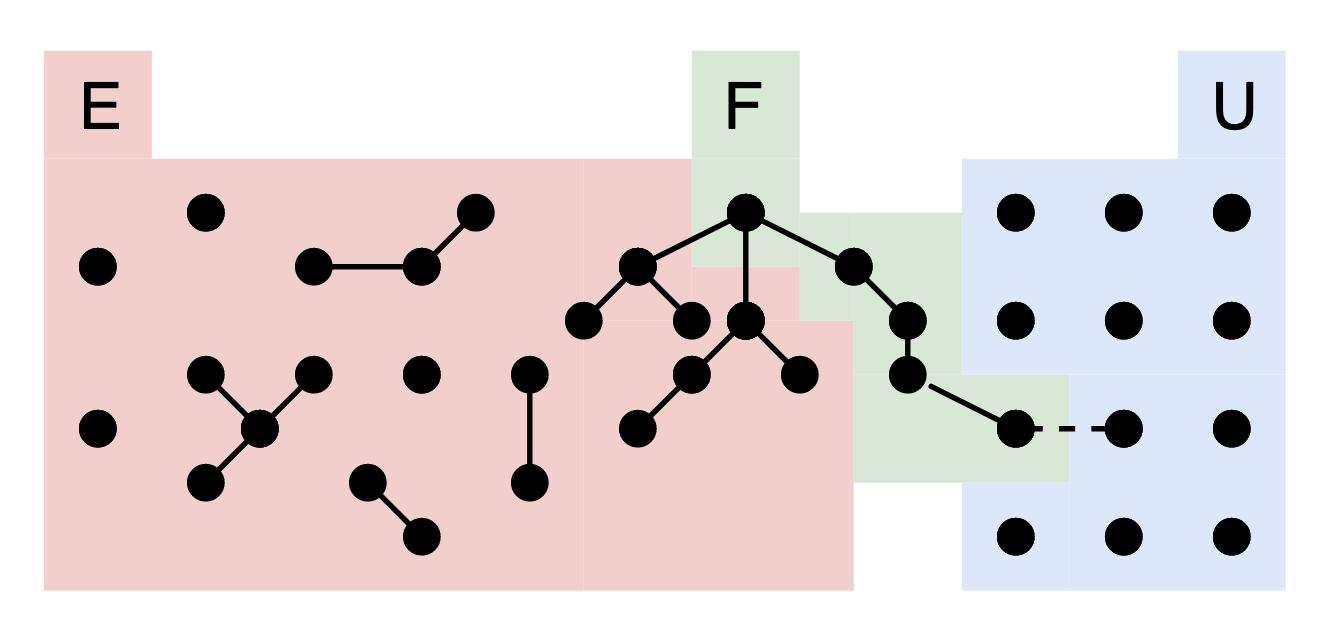
\includegraphics[width=0.75\textwidth]{aulas/10_17/dfs.png}
\end{figure}

\begin{observacao}
  Dado que o valor esperado de queries com resposta positiva é $\delta\,n^2\,p=\delta\left(1+\epsilon\vphantom{1j}\right)$, com probabilidade $\rightarrow1$, temos que o número de respostas positivas é
  \[
    \delta\left(1+\nicefrac{\epsilon}{2}\vphantom{1j}\right)n \leq s \leq \delta\left(1+2\,\epsilon\vphantom{1j}\right)n
  \]
  
  Pela inequação de Chebyshev ou pela de Chernoff.
  
  Sem perda de generalidade, assumiremos $\epsilon\leq\nicefrac{1}{4}$.
\end{observacao}

\begin{fato}
  $\not\exists$ arestas em $G\left(n,\ p\vphantom{1j}\right)$ entre $E$ e $U$, Pelo invariante da DFS.
\end{fato}

Provamos que, se $L_1\left(G\left(n,\ p\vphantom{1j}\right)\vphantom{1j}\right)<\nicefrac{1}{24}\,\epsilon^2\,n$, então $\left|E\vphantom{1j}\right|\,\left|U\vphantom{1j}\right|>t$ no modelo $G_t$.

Isso é uma contradição.

Vamos provar que, em algum momento, $\left|F\vphantom{1j}\right|\geq\nicefrac{1}{24}\,\epsilon^2\,n$, c.c. $\left|E\vphantom{1j}\right|\,\left|U\vphantom{1j}\right|>t$.
% #endregion


\end{document}
